% Assignment 4 - Distributed Matrix Multiplication
% Author: Tomas Santana Suarez
% Compile with pdflatex (Overleaf-ready). Upload this file together with the
% tables/ and figures/ folders. Every table and figure referenced here is
% auto-generated by assignment4/scripts/analyze_results.py and
% collect_system_info.py from the raw measurement CSVs.
\documentclass[11pt,a4paper]{article}

\usepackage[T1]{fontenc}
\usepackage[margin=2.5cm]{geometry}
\usepackage{amsmath,amssymb}
\usepackage{booktabs}
\usepackage{graphicx}
\usepackage{pmboxdraw}
\usepackage{microtype}
\usepackage{caption}
\usepackage{float}
\usepackage[section]{placeins}
\usepackage[hidelinks]{hyperref}

\graphicspath{{figures/}}

\title{\textbf{Distributed Matrix Multiplication}\\with MPI on a Single Host\\
\large Assignment 4 --- Big Data, Grado en Ciencia e Ingeniería de Datos, ULPGC}
\author{Tomás Santana Suárez}
\date{Academic year 2026--2027}

\begin{document}
\maketitle

% =====================================================================
\begin{abstract}
\noindent This study asks how a distributed dense matrix multiplication
scales with the number of workers, and how its end-to-end time splits into
computation, data movement and framework overhead. The product is implemented
in C with MPI (Microsoft MPI) using a 1D row-block partitioning: rank~0
scatters row blocks of $A$, broadcasts $B$, every rank multiplies its rows
with the single-threaded tiled kernel of Assignment~3, and rank~0 gathers $C$.
\emph{All workers are MPI processes on one laptop}, with the instructor's
permission; the results therefore measure process, copy and scheduling
overhead on a shared-memory host, not network performance. For
$n\in\{1000,\dots,4000\}$ and $p\in\{1,2,4,8,16,28\}$ ranks (one warm-up and
five measured repetitions), the speedup over the sequential kernel peaks at
$3.6$--$5.2$ at $p=8$--$16$ and falls to $1.6$--$2.6$ at $p=28$, below the
$6.3$--$8.2$ obtained by the OpenMP kernel of Assignment~3 measured in the
same session. Data movement is a minor cost: at most $8.6\%$ of the
end-to-end time at $n=4000$ and $22.9\%$ at $n=1000$. The loss is dominated
by computation: static equal row blocks cannot balance a hybrid CPU (slowest
to fastest rank up to $2.2\times$), and the $512$-wide tile tuned for one core
performs poorly at $p=28$, consistent with overflowing the shared cache: a
$256$-wide tile makes $p=28$ run $2.9\times$ faster at $n=4000$. Every distributed result is bit-identical to
the single-rank result. Conclusions are scoped to this machine and kernel.
\end{abstract}

% =====================================================================
\section{Introduction and Objective}

Assignments~1--3 built a validated sequential baseline, optimised it with
cache blocking and parallelised it with OpenMP threads on a single
shared-memory machine. A distributed implementation changes the programming
model: every worker owns its memory and data moves only through explicit
messages, which adds copies, synchronisation and framework start-up costs on
top of the computation. This study measures how much those costs matter and
how the distributed version compares with the shared-memory one.

\paragraph{Research question.} \emph{How does an MPI row-block matrix
multiplication scale with the number of workers $p$, and what share of its
end-to-end time is computation, data transfer and framework overhead,
compared with the sequential kernel and the OpenMP kernel of Assignment~3?}

\paragraph{Factors and metrics.} Independent factors: worker count
$p\in\{1,2,4,8,16,28\}$ (MPI ranks, one single-threaded process each) and
size $n\in\{1000,2000,3000,4000\}$, where $n$ is the side length of a square
matrix. Metrics: end-to-end time, its four phases, strong-scaling speedup
$S(p)=T_{\mathrm{seq}}(n)/T_p(n)$, efficiency $E(p)=S(p)/p$ (both from
\emph{median} times) and memory per rank. The problem size is fixed while
$p$ grows (strong scaling); weak scaling is not studied.

\paragraph{Local Execution Limitation.} With the instructor's permission,
all ranks run on \textbf{one laptop}: 28 logical processors, one RAM and one
last-level cache, exchanging data through the shared-memory transport of the
MPI runtime. The experiment can show framework, copy and process-scheduling
behaviour. It does \emph{not} show inter-machine network bandwidth or latency,
nor multi-machine memory capacity, and ``workers'' are processes, not
machines. No network measurement is claimed anywhere in this report.

\paragraph{Hypotheses (stated before measuring).}
\textbf{H1:} at equal worker count the MPI version is not faster than the
OpenMP version, because it adds the scatter, the broadcast of a full copy of
$B$ to every rank and the gather. \textbf{H2:} the share of data movement in
the end-to-end time grows with $p$ and shrinks with $n$. \textbf{H3:} small
$n$ is dominated by overhead, so its speedup saturates early.
\textbf{H4:} the compute phase scales like the Assignment~3 kernel, since it
is the same kernel on a fraction of the rows.

% =====================================================================
\section{Background and References}

\subsection{Message passing and collectives}
MPI~\cite{mpi22} is the standard message-passing interface for distributed
memory: processes (ranks) with private address spaces cooperate through
point-to-point and collective operations~\cite{gropp2014}. The collectives
used here are \texttt{MPI\_Scatterv} (distinct blocks to each rank),
\texttt{MPI\_Bcast} (the same data to all) and \texttt{MPI\_Gatherv}
(blocks back to one rank); their cost depends on message size, rank count and
the algorithm chosen by the library~\cite{thakur2005}. The runtime used is
Microsoft MPI~\cite{msmpi}.

\subsection{Partitioning dense products}
In a 1D row-block scheme each rank computes a band of rows of $C=AB$ and needs
the corresponding band of $A$ and \emph{all} of $B$, so memory per rank is
$\Theta(n^2)$ regardless of $p$ and the data sent grows linearly with $p$.
2D block schemes such as SUMMA~\cite{vandegeijn1997} bound per-rank memory by
$\Theta(n^2/p)$ and reduce communication volume at the price of a more complex
algorithm. The row-block scheme was chosen for its simplicity and because the
accumulation order of every $C_{ij}$ does not depend on the split.

\subsection{Scaling laws and the memory hierarchy}
Amdahl's law~\cite{amdahl1967} bounds speedup by the serial fraction of a
fixed workload (strong scaling), and Gustafson~\cite{gustafson1988} describes
scaled workloads. Dense multiplication has almost no serial computation, so
the limits are shared hardware resources, as formalised by the roofline
model~\cite{williams2009}. Cache blocking~\cite{lam1991,goto2008} keeps a tile
in fast memory, and its best size depends on the cache capacity available to
each worker, which shrinks as more workers share a last-level
cache~\cite{hennessy2017}. The test CPU is hybrid: performance cores (P-cores)
with two hardware threads each and slower efficiency cores (E-cores).

% =====================================================================
\section{Methodology}\label{sec:method}

\subsection{Implementation (custom student code in C)}
\paragraph{Partitioning.} Rank~0 owns the full $A$, $B$, $C$. \texttt{MPI\_Scatterv}
sends rank $r$ a contiguous block of $\lceil n/p\rceil$ or $\lfloor n/p\rfloor$
rows of $A$ (the $n \bmod p$ remainder rows go to the first ranks, so block
sizes differ by at most one row); \texttt{MPI\_Bcast} sends the whole of $B$ to
every rank; each rank multiplies its rows; \texttt{MPI\_Gatherv} collects the
row blocks of $C$ on rank~0. Rank~0 works in place (its block is the first
rows of $A$ and $C$), non-root ranks allocate and touch their buffers before
the timer starts, and ranks owning no row ($p>n$) take part in every
collective with empty blocks.

\paragraph{Local kernel.} The compute step is the Assignment~3 tiled
$i$-$k$-$j$ kernel generalised from $n\times n$ to a row block, compiled once
with \texttt{-O3 -march=native} (vectorised, no OpenMP), tiles of $16$ rows
$\times$ $512$ columns, i.e.\ the same tile shape as the Assignment~3 parallel
runs. The kernel never calls MPI. Every $C_{ij}$ accumulates its $n$ products
in ascending $k$ order whatever the split, so the distributed $C$ must be
bit-identical to the single-rank $C$.

\paragraph{Architecture.} A \texttt{Partitioner} interface (create, multiply,
destroy, storage size) hides the scheme from the harness; the row-block scheme
is one registered implementation, so a 2D scheme could be added without
touching the harness. Workers are single-threaded processes: the worker count
is exactly the number of ranks, no numerical library is linked and OpenMP is
not used.

\paragraph{Baselines.} The Assignment~3 sequential kernel and OpenMP kernel
are re-run in the same measurement session, immediately before the MPI runs,
at the same sizes and worker counts (OpenMP threads for $p$), so that thermal
and operating-system conditions are shared. They are different programs
(threads versus processes, one shared $B$ versus one private copy per rank),
which prevents a perfectly isolated comparison; the differences are discussed
rather than hidden.

\subsection{Inputs}
The Assignment~1 matrices are reused unchanged (float64, uniform in
$[-10,10]$, Mersenne Twister seed 42); \texttt{scripts/generate\_matrices.py}
recreates them bit-identically. Sizes $1000$--$4000$ overlap with
Assignments~1--3, as required for the comparison. Rank~0 loads $A_n$, $B_n$
from CSV before the timer; the other ranks start empty.

\subsection{Environment and process placement}\label{sec:env}
Table~\ref{tab:env} is generated by \texttt{collect\_system\_info.py}; the core
topology is read at run time, not typed by hand. Assignment~3 showed that
Windows may place single-thread runs on E-cores and distort speedups, so every
rank opts out of EcoQoS power throttling and the single-rank run is restricted
to the P-cores; for $p\ge2$ placement is left to the Windows scheduler.
\texttt{mpiexec -affinity} was tested as an alternative and made the runs
slower (Section~\ref{sec:probes}), so it is not used.

% Auto-generated by scripts/collect_system_info.py -- do not edit.
\begin{table}[H]
\centering
\small
\caption{Benchmarking machine and toolchain (single host).}
\label{tab:env}
\begin{tabular}{lp{0.68\linewidth}}
\toprule
Component & Value \\
\midrule
CPU model & Intel(R) Core(TM) i7-14700HX \\
Core topology & 20 cores / 28 logical: 8 P-cores (16 logical, SMT) + 12 E-cores (12 logical) \\
Last-level cache (L3) & 33 MB \\
Total RAM & 31,7 GB \\
Operating system & Windows 11 (build 10.0.26300) \\
Power plan & High performance (8c5e7fda-e8bf-4a96-9a85-a6e23a8c635c) \\
C compiler & gcc (Rev4, Built by MSYS2 project) 16.2.0 \\
Kernel flags & -O3 -march=native (vectorised, no OpenMP) \\
SIMD target & AVX2=1, FMA=1, AVX-512F=0 \\
MPI runtime & Microsoft MPI (MS-MPI), MPI standard 2.0; Microsoft MPI 10.1.12498.52 \\
Execution model & one single-threaded MPI process per worker; all ranks on one host (local execution, shared-memory transport of MS-MPI) \\
Placement & EcoQoS opt-out in every rank; p=1 pinned to P-cores; p>=2 scheduled by Windows over the 28 logical processors \\
Library threads & no numerical library linked; OMP\_NUM\_THREADS=(unset) \\
Analysis runtime & CPython 3.11.9 \\
\bottomrule
\end{tabular}
\end{table}


\subsection{Timing boundary, repetitions, memory and budgets}
\paragraph{End-to-end boundary.} Time starts when $A$ and $B$ are in rank-0
memory and stops when $C$ is in rank-0 memory: scatter $+$ broadcast $+$
compute $+$ gather, measured on rank~0 with
\texttt{clock\_gettime(CLOCK\_MONOTONIC)} between barriers. The four phases
are consecutive intervals of one clock, so within each run they add up to the
total; the barriers make the phases separable but remove any overlap between
them, so the phase shares describe this instrumented execution. The compute
phase is the slowest rank's time (plus a four-byte completion agreement). The
fastest and slowest rank's kernel time are gathered \emph{after} the boundary
and expose load imbalance. Outside the boundary and reported separately:
reading the CSV inputs and the start-up of the MPI processes (launcher wall
clock of \texttt{mpiexec} for a program that only initialises and finalises
MPI). The sequential and OpenMP baselines time the kernel with data already in
memory; at $p=1$ the distributed run performs exactly the same operations (no
data movement), so $S(p)$ compares equivalent boundaries.

\paragraph{Repetitions and statistics.} Each configuration runs one warm-up
(excluded) and $N=5$ measured repetitions; the trace of $C$ is logged after
every run so the computation cannot be eliminated. Medians and interquartile
ranges (IQR) are reported; $S(p)$ and $E(p)$ use medians, and the speedup error
bars propagate the IQR of $T_p$ with $T_{\mathrm{seq}}$ fixed at its median.
Diagnostic probes use $N=3$ and are labelled as such.

\paragraph{Memory and budgets.} The metric is the peak process working set
(resident memory) of each rank, sampled every $5$\,ms; it is reported as the
sum over ranks, for rank~0 and for the largest non-root rank, next to the
theoretical matrix storage of the scheme. Rank~0 additionally holds the
harness' reference result. Process resident memory must not be compared with
managed-heap measures of other runtimes. Budget: $120$\,s per run (collective
watchdog; a timeout would be logged as \texttt{TIMEOUT} with no time) and
about $4.3$\,GiB of resident memory in total at $n=4000$, $p=28$, well within
the installed RAM (Table~\ref{tab:env}). Every configuration completed within budget.

\subsection{Correctness}
A gate of 43 checks runs before every benchmark launch and aborts all ranks on
failure: $A\times I=A$ and $A\times0=0$ for $n\in\{1,2,4,8,16\}$, a known
$2\times2$ product, and agreement with an independent $k$-$i$-$j$ reference for
$n\in\{1,2,4,8,16,17,33,100\}$ with default tiles and with tiny tiles
($3\times8$) that exercise every remainder path. The gate was run with
$p\in\{1,2,3,4,7,8,16,28\}$ ranks, which includes $p>n$ (ranks without rows)
and $n$ not divisible by $p$ (uneven \texttt{Scatterv}/\texttt{Gatherv}
counts). Tolerances are $\epsilon_{\mathrm{abs}}=\epsilon_{\mathrm{rel}}=
10^{-9}$ as in Assignment~3, and the distributed result must also be
\textbf{bit-identical} (\texttt{memcmp}) to the single-block result of the same
kernel. During the benchmark every configuration was compared bitwise with a
single-rank reference computed on rank~0 outside the timer (24 of 24
identical in the main experiment), and an external NumPy check at $n=1000$,
$p=28$ gave $\max|C-C_{\mathrm{NumPy}}|=1.4\times10^{-11}$.

% =====================================================================
\section{Results}\label{sec:results}

\subsection{Scaling versus the sequential and OpenMP kernels}
Table~\ref{tab:time} lists every median and IQR, Table~\ref{tab:speedup} the
speedup and efficiency of the MPI version next to the OpenMP kernel measured in
the same session, and Figures~\ref{fig:time} and~\ref{fig:speedup} show them
against $p$.

% Auto-generated by scripts/analyze_results.py -- do not edit.
\begin{table}[H]
\centering
\small
\caption{End-to-end time of the distributed product in ms (median [IQR], $N=5$ measured repetitions, 1 warm-up excluded) for $p$ MPI ranks on one host, versus the sequential kernel measured in the same session. End-to-end = $A,B$ in rank-0 memory $\rightarrow$ $C$ in rank-0 memory.}
\label{tab:time}
\begin{tabular}{lrrrr}
\toprule
Configuration & $n=1000$ & $n=2000$ & $n=3000$ & $n=4000$ \\
\midrule
Sequential (A3 kernel) & 79.2 [2.0] & 826.4 [1.5] & 3{,}082 [143] & 7{,}090 [421] \\
\midrule
MPI $p=1$ & 83.1 [0.8] & 841.6 [15.0] & 2{,}886 [152] & 6{,}757 [65] \\
MPI $p=2$ & 46.7 [0.6] & 445.2 [1.0] & 1{,}529 [4] & 3{,}661 [13] \\
MPI $p=4$ & 27.7 [0.9] & 261.6 [2.1] & 879.4 [4.1] & 2{,}111 [31] \\
MPI $p=8$ & 22.0 [0.6] & 184.3 [0.1] & 615.6 [1.8] & 1{,}420 [21] \\
MPI $p=16$ & 31.2 [3.8] & 202.2 [6.7] & 592.9 [17.5] & 1{,}365 [66] \\
MPI $p=28$ & 49.9 [0.1] & 333.7 [9.8] & 1{,}189 [175] & 2{,}807 [32] \\
\bottomrule
\end{tabular}
\end{table}


\begin{figure}[H]
\centering
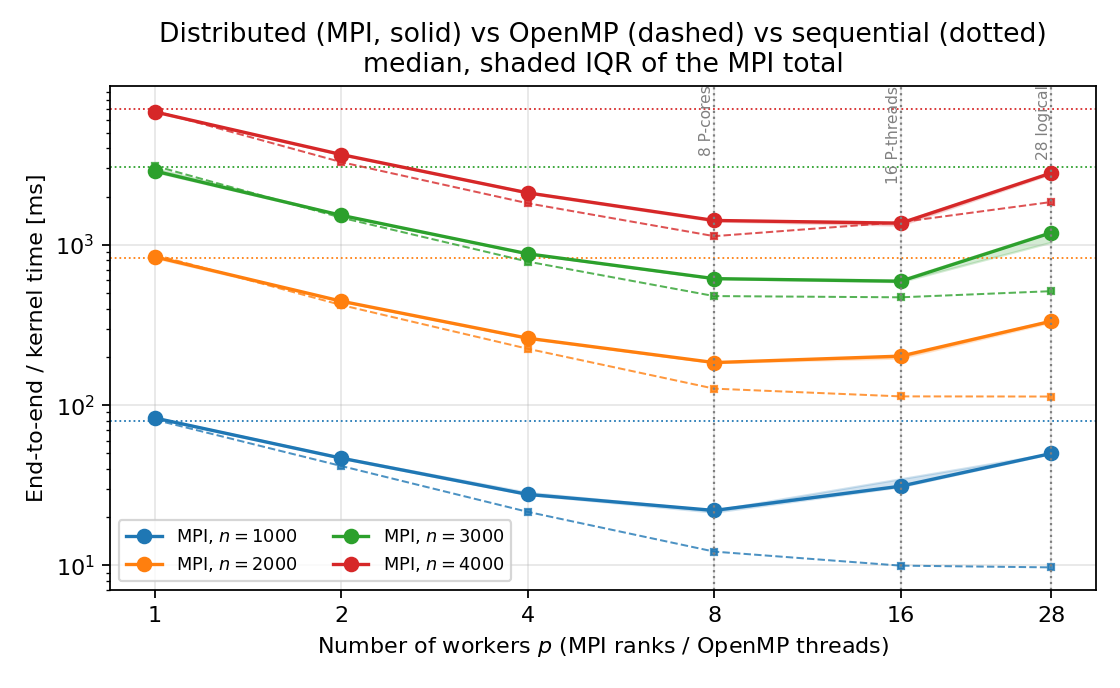
\includegraphics[width=0.82\linewidth]{fig_time_vs_workers.png}
\caption{End-to-end time of the MPI version (solid, shaded IQR), kernel time
of the Assignment~3 OpenMP version in the same session (dashed) and the
sequential kernel (dotted), log--log, medians. Dotted vertical guides: 8
P-cores, 16 P-core hardware threads, 28 logical processors.}
\label{fig:time}
\end{figure}

% Auto-generated by scripts/analyze_results.py -- do not edit.
\begin{table}[H]
\centering
\small
\caption{Strong-scaling speedup $S(p)=T_{\mathrm{seq}}(n)/T_p(n)$ (efficiency $E(p)=S(p)/p$ in parentheses), from median times. Each cell: MPI row-block / Assignment~3 OpenMP kernel measured in the same session.}
\label{tab:speedup}
\begin{tabular}{lcccc}
\toprule
$p$ & $n=1000$ & $n=2000$ & $n=3000$ & $n=4000$ \\
\midrule
1 & 0.95 (0.95) / 0.98 & 0.98 (0.98) / 0.95 & 1.07 (1.07) / 0.99 & 1.05 (1.05) / 1.03 \\
2 & 1.70 (0.85) / 1.90 & 1.86 (0.93) / 1.96 & 2.02 (1.01) / 2.09 & 1.94 (0.97) / 2.16 \\
4 & 2.86 (0.71) / 3.67 & 3.16 (0.79) / 3.68 & 3.50 (0.88) / 3.92 & 3.36 (0.84) / 3.90 \\
8 & 3.60 (0.45) / 6.50 & 4.48 (0.56) / 6.52 & 5.01 (0.63) / 6.43 & 4.99 (0.62) / 6.26 \\
16 & 2.54 (0.16) / 7.95 & 4.09 (0.26) / 7.29 & 5.20 (0.32) / 6.55 & 5.19 (0.32) / 5.12 \\
28 & 1.59 (0.06) / 8.15 & 2.48 (0.09) / 7.30 & 2.59 (0.09) / 6.00 & 2.53 (0.09) / 3.83 \\
\bottomrule
\end{tabular}
\end{table}


\begin{figure}[H]
\centering
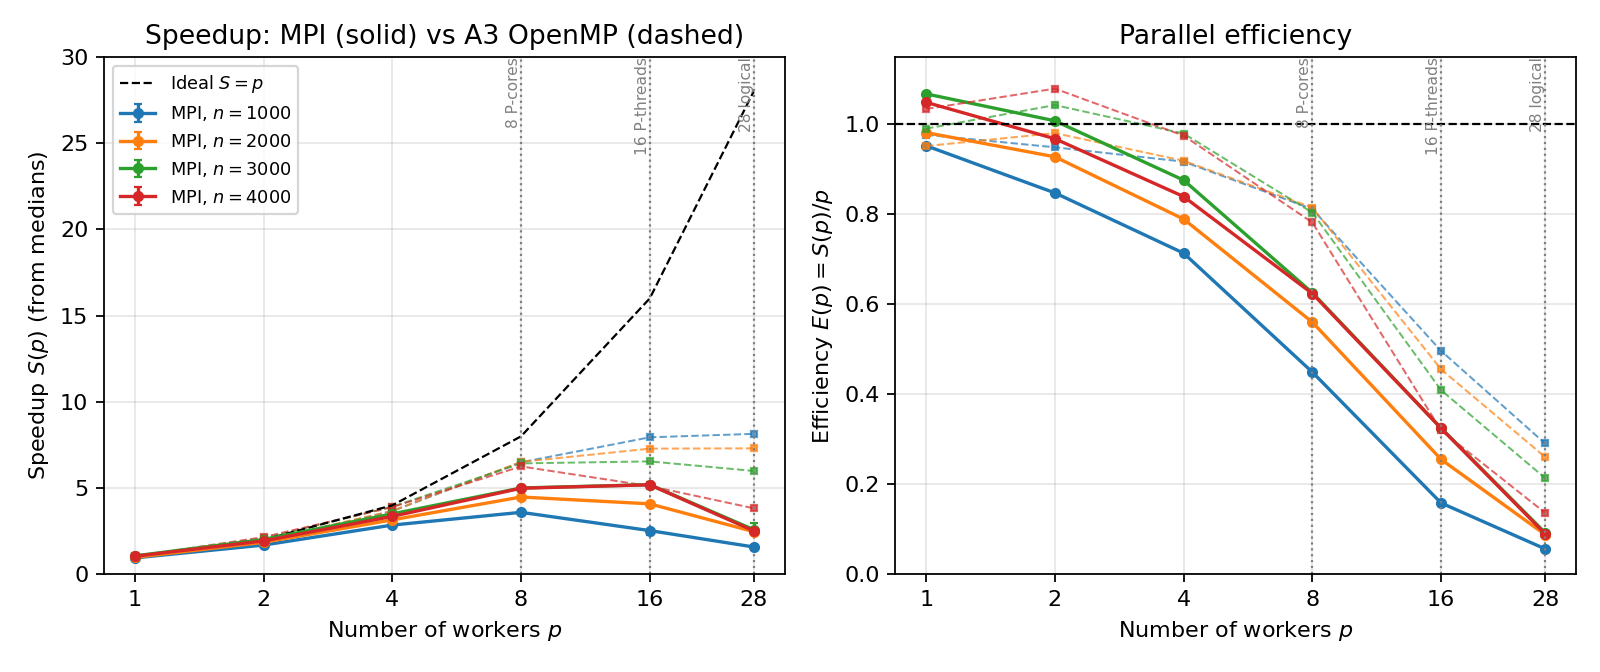
\includegraphics[width=\linewidth]{fig_speedup_efficiency.png}
\caption{Speedup (left, with ideal $S=p$) and efficiency (right) from median
times; solid: MPI, dashed: OpenMP kernel of Assignment~3. Error bars: range of
$S$ induced by the IQR of $T_p$.}
\label{fig:speedup}
\end{figure}

With one rank the distributed program takes $0.94$--$1.05\times$ the
sequential time ($79.2$, $826$, $3082$, $7090$\,ms for $n=1000,\dots,4000$);
the differences are comparable to the IQR of the sequential baseline
($143$ and $421$\,ms at $n=3000$ and $4000$) and there is no data movement at
$p=1$. For $p\le4$ scaling is good ($S(4)=2.86$--$3.50$, $E\ge0.71$). The
best speedups are $3.60$ ($n=1000$, $p=8$), $4.48$ ($n=2000$, $p=8$), $5.20$
($n=3000$, $p=16$) and $5.19$ ($n=4000$, $p=16$). At $p=28$ the speedup
collapses to $1.59$--$2.59$ ($E=0.06$--$0.09$), and for $n=4000$ the end-to-end
time is $2.81$\,s, twice the $1.37$\,s of $p=16$. The OpenMP kernel reaches
$S(8)=6.26$--$6.52$ and a best of $6.26$--$8.15$. The MPI time exceeds the
OpenMP time by $1.25$--$1.81\times$ at $p=8$ and by $1.52$--$5.14\times$ at
$p=28$; the only tie is $n=4000$, $p=16$ (ratio $0.99$).

\subsection{Phase decomposition and data movement}
% Auto-generated by scripts/analyze_results.py -- do not edit.
\begin{table}[H]
\centering
\small
\caption{Phase decomposition at $n=4000$ (median ms over $N=5$ repetitions). The phases are consecutive barrier-delimited intervals of one clock, so within each run they add up to the end-to-end time (medians of the phases need not add up exactly to the median total); the barriers remove any overlap between phases. Kernel min/max are the fastest and slowest rank's compute time, measured outside the boundary.}
\label{tab:phases-large}
\begin{tabular}{rrrrrrrrr}
\toprule
$p$ & Scatter & Bcast & Compute & Gather & Total & Comm.\ share & Kernel min & Kernel max \\
\midrule
1 & 0.0 & 0.0 & 6757.1 & 0.0 & 6757.1 & 0.0\% & 6757.1 & 6757.1 \\
2 & 6.5 & 12.7 & 3635.1 & 6.5 & 3660.8 & 0.7\% & 3625.1 & 3635.1 \\
4 & 10.8 & 30.4 & 2059.3 & 9.9 & 2110.7 & 2.4\% & 2042.6 & 2059.3 \\
8 & 12.6 & 46.7 & 1349.3 & 11.8 & 1420.0 & 5.0\% & 1313.2 & 1349.0 \\
16 & 14.6 & 89.8 & 1245.6 & 13.2 & 1365.4 & 8.6\% & 792.4 & 1245.4 \\
28 & 21.9 & 149.6 & 2610.7 & 18.9 & 2806.8 & 6.8\% & 2265.7 & 2614.1 \\
\bottomrule
\end{tabular}
\end{table}


\begin{figure}[H]
\centering
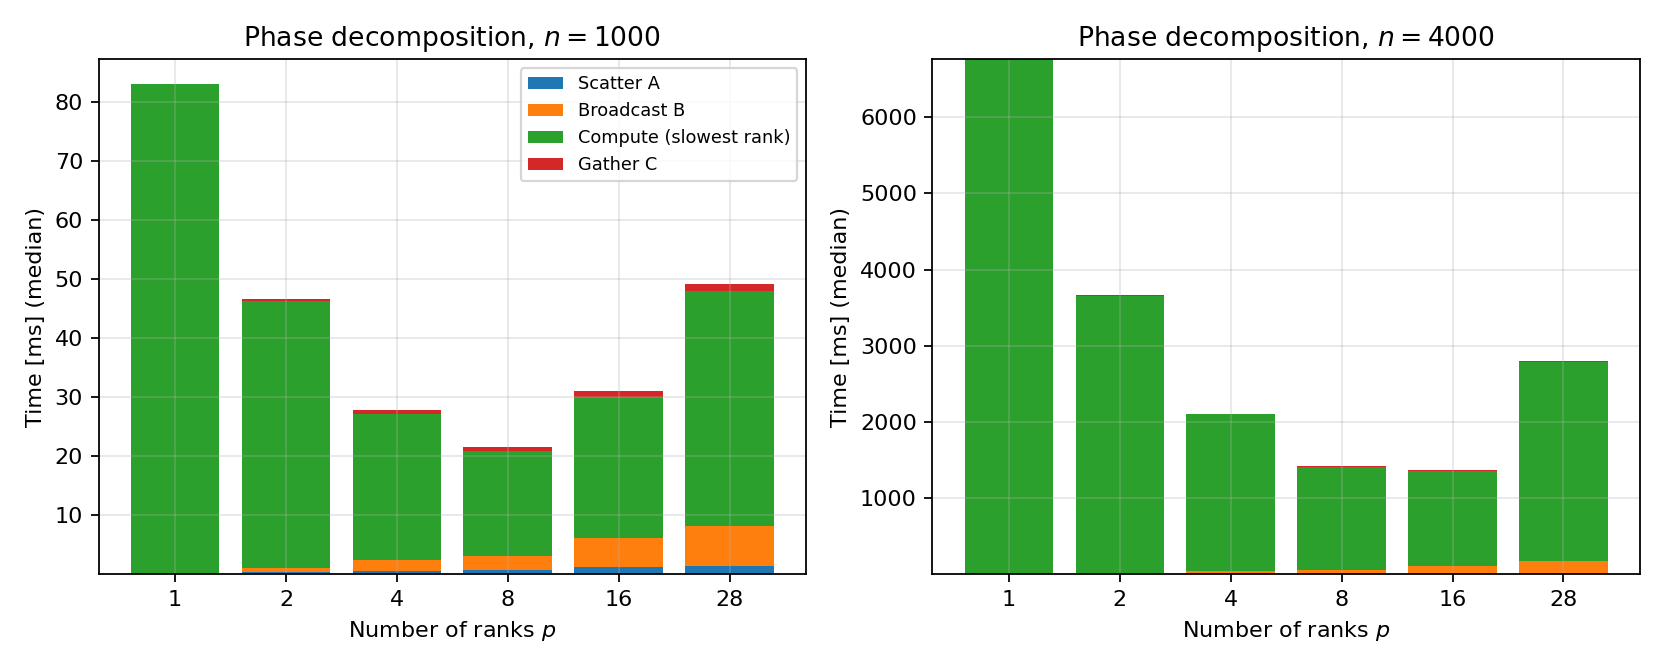
\includegraphics[width=\linewidth]{fig_phases.png}
\caption{Phase decomposition of the end-to-end time (median) for the smallest
and largest size.}
\label{fig:phases}
\end{figure}

% Auto-generated by scripts/analyze_results.py -- do not edit.
\begin{table}[H]
\centering
\small
\caption{Share of the end-to-end time spent in data movement (scatter $+$ broadcast $+$ gather), in percent of the median total.}
\label{tab:commshare}
\begin{tabular}{lrrrr}
\toprule
$p$ & $n=1000$ & $n=2000$ & $n=3000$ & $n=4000$ \\
\midrule
1 & 0.0 & 0.0 & 0.0 & 0.0 \\
2 & 3.1 & 1.4 & 0.9 & 0.7 \\
4 & 10.9 & 5.1 & 3.3 & 2.4 \\
8 & 17.9 & 9.9 & 6.4 & 5.0 \\
16 & 22.9 & 16.2 & 11.9 & 8.6 \\
28 & 18.8 & 14.3 & 8.8 & 6.8 \\
\bottomrule
\end{tabular}
\end{table}


Data movement stays small (Table~\ref{tab:commshare}). At $n=4000$ scatter,
broadcast and gather add up to $25.7$\,ms at $p=2$ and $190$\,ms at $p=28$
($0.7\%$ to $6.8\%$ of the total, at most $8.6\%$ at $p=16$); the broadcast is
$79\%$ of it at $p=28$ ($150$\,ms for $27$ copies of the $128$\,MB matrix $B$,
an aggregate copy rate of about $23$\,GB/s, derived from the measurement). At
$n=1000$ the share is larger ($3.1\%$ at $p=2$, $22.9\%$ at $p=16$, $18.8\%$ at
$p=28$) and at every size it grows up to $p=16$; it falls at $p=28$ only
because the compute phase grows. The compute phase dominates everywhere:
$91$--$100\%$ of the total at $n=4000$. Its spread across ranks is the key
anomaly: the slowest-to-fastest ratio of the per-rank kernel time is
$\le1.05$ for $p\le8$ but $1.57$--$2.18$ at $p=16$ (at $n=4000$: $792$\,ms
versus $1246$\,ms) and $1.15$--$1.37$ at $p=28$.

\subsection{Memory and costs outside the boundary}
% Auto-generated by scripts/analyze_results.py -- do not edit.
\begin{table}[H]
\centering
\small
\caption{Memory at $n=4000$. Metric: peak process working set (resident memory) of each MPI rank, sampled every 5\,ms. Sum over ranks, rank 0 (owns $A$, $B$, $C$ and the harness' reference result) and the largest non-root rank (its $B$ copy plus its row blocks of $A$ and $C$), versus the theoretical matrix storage allocated by the strategy (all values in MB, median).}
\label{tab:memory}
\begin{tabular}{rrrrr}
\toprule
$p$ & Sum over ranks & Rank 0 & Max non-root rank & Theoretical sum \\
\midrule
1 & 497 & 497 & -- & 366 \\
2 & 750 & 497 & 253 & 610 \\
4 & 1073 & 497 & 192 & 916 \\
8 & 1634 & 498 & 163 & 1434 \\
16 & 2696 & 498 & 147 & 2426 \\
28 & 4274 & 498 & 140 & 3898 \\
\bottomrule
\end{tabular}
\end{table}


% Auto-generated by scripts/analyze_results.py -- do not edit.
\begin{table}[H]
\centering
\small
\caption{Costs outside the end-to-end boundary. Left: launcher wall clock of \texttt{mpiexec -n p} for a program that only initialises and finalises MPI (median [IQR] of $N=5$ launches, ms). Right: rank-0 time to read $A_n$ and $B_n$ from CSV (median ms).}
\label{tab:overheads}
\begin{tabular}{rr@{\qquad}rr}
\toprule
$p$ & MPI start-up & $n$ & CSV load \\
\midrule
1 & 36.2 [0.4] & 1000 & 338 \\
2 & 39.1 [0.9] & 2000 & 1{,}326 \\
4 & 42.2 [1.1] & 3000 & 2{,}961 \\
8 & 60.1 [0.4] & 4000 & 5{,}228 \\
16 & 92.6 [0.4] &  &  \\
28 & 146.0 [3.9] &  &  \\
\bottomrule
\end{tabular}
\end{table}


Memory values are in MiB ($2^{20}$ bytes), labelled MB in the tables. At
$n=4000$ the summed working set grows from $497$ ($p=1$) to $4274$ ($p=28$),
about one extra copy of $B$ ($122$ MiB plus process overhead) per rank, while
the largest non-root rank falls from $253$ to $140$ and rank~0 stays at about
$498$ (it owns $A$, $B$, $C$ and the reference result).
Starting the processes costs $36$\,ms at $p=1$ and $146$\,ms at $p=28$, and
reading the CSV inputs costs $0.34$--$5.2$\,s, far more than the end-to-end
time itself at large $n$ (best $1.37$\,s at $n=4000$): including it would hide
everything this study measures, which is why it is outside the boundary.

\subsection{Diagnostic probes}\label{sec:probes}
Two small probes test explanations of the large-$p$ behaviour ($N=3$, not part
of the main statistics).

% Auto-generated by scripts/analyze_results.py -- do not edit.
\begin{table}[H]
\centering
\small
\caption{Probe of the large-$p$ slowdown: end-to-end time in ms (median [IQR]) with the Assignment~2/3 tuned $512$-wide $k/j$ tile (main experiment, $N=5$) and with a $256$-wide tile (diagnostic probe, $N=3$), same code and inputs. Gain $=T_{512}/T_{256}$.}
\label{tab:probe}
\begin{tabular}{rrrrr}
\toprule
$n$ & $p$ & $512$-wide tile & $256$-wide tile & Gain \\
\midrule
2000 & 8 & 184.3 [0.1] & 133.4 [1.6] & 1.38 \\
2000 & 16 & 202.2 [6.7] & 139.5 [1.2] & 1.45 \\
2000 & 28 & 333.7 [9.8] & 149.3 [2.0] & 2.23 \\
4000 & 8 & 1{,}420 [21] & 980.8 [6.5] & 1.45 \\
4000 & 16 & 1{,}365 [66] & 926.5 [3.0] & 1.47 \\
4000 & 28 & 2{,}807 [32] & 954.4 [13.3] & 2.94 \\
\bottomrule
\end{tabular}
\end{table}


% Auto-generated by scripts/analyze_results.py -- do not edit.
\begin{table}[H]
\centering
\small
\caption{Diagnostic of \texttt{mpiexec -affinity} (MS-MPI default pinning layout, $N=3$) against the default Windows scheduling of the main experiment ($N=5$): end-to-end time in ms (median [IQR]) and ratio of the slowest to the fastest rank's kernel time.}
\label{tab:affinity}
\begin{tabular}{rrrrrr}
\toprule
$n$ & $p$ & Default & Imbalance & \texttt{-affinity} & Imbalance \\
\midrule
2000 & 8 & 184.3 [0.1] & 1.04 & 241.1 [47.0] & 1.53 \\
2000 & 16 & 202.2 [6.7] & 1.65 & 224.0 [2.9] & 1.79 \\
4000 & 8 & 1{,}420 [21] & 1.03 & 1{,}869 [36] & 1.52 \\
4000 & 16 & 1{,}365 [66] & 1.57 & 1{,}590 [44] & 1.77 \\
\bottomrule
\end{tabular}
\end{table}


Table~\ref{tab:probe} repeats the MPI runs with a $256$-wide instead of
$512$-wide $k/j$ tile (same code and inputs). At $p=28$ the time falls from
$2.81$ to $0.95$\,s at $n=4000$ ($2.94\times$) and from $334$ to $149$\,ms at
$n=2000$ ($2.23\times$); at $p=8$--$16$ the gain is $1.4$--$1.5\times$.
Table~\ref{tab:affinity} shows that pinning the ranks with
\texttt{mpiexec -affinity} (MS-MPI default layout) is worse than the default
scheduling and creates imbalance even at $p=8$ (ratio $1.52$ versus $1.03$).

% =====================================================================
\section{Discussion}\label{sec:disc}

\subsection{Answer to the research question}
On this host the MPI row-block product scales well to $p=4$ and reaches a
speedup of $3.6$--$5.2$ at $p=8$--$16$, after which it degrades; it is
slower than the OpenMP kernel at equal $p$, and the gap widens with $p$ and
shrinks with $n$. Computation, not data transfer, is the dominant cost
(Figure~\ref{fig:phases}): data movement is $\le8.6\%$ of the end-to-end time
for $n=4000$ and $\le22.9\%$ for $n=1000$, framework start-up is
$36$--$146$\,ms and is outside the boundary, and the rest is a compute phase
that stops scaling. The losses therefore come from how the processes use the
shared hardware, which is a property of local execution; they say little about
what a cluster would show.

\subsection{Hypotheses}
\textbf{H1} is confirmed for $p\ge2$ (MPI/OpenMP time ratio $1.03$--$5.14$,
with one tie at $n=4000$, $p=16$), but the mechanism is not the copies: at
$n=4000$ data movement is only $0.7$--$8.6\%$, yet the MPI compute phase is
already $13\%$ slower than the OpenMP kernel at $p=4$ ($2059$ versus
$\approx1818$\,ms, derived from $S_{\mathrm{OpenMP}}(4)=3.90$) where the rank
imbalance is only $1.01$. A plausible, untested contributor is that OpenMP
threads share one copy of $B$ and tend to sweep the same panels together,
whereas each rank streams a private copy. \textbf{H2} is confirmed: the share
of data movement grows with $p$ up to $16$ and shrinks with $n$ ($22.9\%$,
$16.2\%$, $11.9\%$, $8.6\%$ at $p=16$), with the drop at $p=28$ explained
above. \textbf{H3} is confirmed: at $n=1000$ the best speedup is only $3.60$,
the time at $p=28$ ($49.9$\,ms) is worse than at $p=4$ ($27.7$\,ms) and data
movement reaches $22.9\%$. \textbf{H4} holds only approximately for $p=2$ (compute-phase speedup $1.95$
against $2.16$ for the OpenMP kernel at $n=4000$) and fails from $p=4$,
for the reasons below.

\subsection{Why compute stops scaling}
\paragraph{Static partitioning on a hybrid CPU.} Each rank receives the same
number of rows, so the compute phase equals the slowest rank. With $p\le8$ the
ranks run at the same speed (ratio $\le1.05$); at $p=16$ some ranks share a
P-core through SMT or land on slower E-cores and need up to $2.2\times$ longer
than the fastest, so the end-to-end time is set by them (at $n=4000$, $p=16$
the fastest rank finishes in $792$\,ms but the phase lasts $1246$\,ms). OpenMP's
dynamic scheduling in Assignment~3 avoided this by giving slow threads fewer
tiles. The actual placement of ranks on cores was not observed, so which cores
the slow ranks use is an inference from the ratios, not a measurement.

\paragraph{Shared-cache capacity.} At $p=28$ even the fastest rank needs
$2266$\,ms at $n=4000$ (ideal share: $7090/28\approx253$\,ms), so imbalance
cannot be the whole story. The same $512$-wide tile that was tuned for one
core in Assignment~2 was shown in Assignment~3 to degrade runs with many
workers, an effect attributed there to the shared L3 being overflowed when
workers stream different panels at once; here the $256$-wide tile makes
$p=28$ run $2.94\times$ faster (Table~\ref{tab:probe}), the same signature and
a similar magnitude as in Assignment~3 ($2.8\times$ for OpenMP). Against the
$512$-tile sequential baseline this corresponds to $S=7.4$, but that figure
overstates the benefit because a sequential baseline with the $256$-wide tile
was not measured here (in Assignment~3, a different session, the sequential
kernel itself was faster with that tile), so only the gain $T_{512}/T_{256}$
is a like-for-like result. For the MPI version the effect is likely larger
because the ranks' private copies of $B$ prevent any sharing of cached
panels, which is a hypothesis, not a result.

\subsection{What this does and does not say about distribution}
The observed broadcast cost, about $0.15$\,s for $27$ copies of $B$ at
$n=4000$, is the cost of memory-to-memory copies on one host. A real network
would pay the same volume ($\Theta(p\,n^2)$ for this scheme) at the bandwidth
and latency of the interconnect, so data movement would very probably take a
larger share; no number for that case can be derived from these data, and
none is claimed. The row-block scheme also replicates $B$ on every rank
(Table~\ref{tab:memory}), so it does not increase the largest problem a
cluster could hold; the 2D schemes of Section~2 would.

\subsection{Anomalies and limitations}
(i) One host: placement of ranks for $p\ge2$ is decided by Windows and could not
be controlled (\texttt{-affinity} made it worse), and ratios such as the
$p=16$ imbalance depend on that. (ii) The diagnostic probes use $N=3$ and one
or two sizes. (iii) The barriers separate the phases but remove any overlap, so
the decomposition is that of the instrumented run. (iv) The baselines come from
a different program (OpenMP threads); the sequential baseline has a noticeable
IQR at $n=3000$ and $4000$ ($143$ and $421$\,ms), so speedups within about
$\pm6\%$ of each other are not distinguishable. (v) Only static row-block
partitioning was implemented; dynamic distribution or 2D schemes might behave
differently. (vi) Memory is process resident memory including harness
buffers on rank~0. (vii) Configurations ran in a fixed order, so slow thermal
drift cannot be excluded. (viii) The MPI runtime reports MPI standard 2.0;
only basic collectives are used.

% =====================================================================
\section{Conclusions}

Within the tested scope (C + MS-MPI, float64, row-block partitioning with a
broadcast $B$, $n\le4000$, $p\le28$ ranks \emph{on one laptop}, local
execution permitted by the instructor):

\begin{enumerate}
\item The distributed product is correct and deterministic: bit-identical to
the single-rank result in all 24 benchmark configurations and in the 43-check
gate for eight rank counts, including ranks without rows.
\item Strong scaling is good up to $p=4$, peaks at $S=3.6$--$5.2$ for
$p=8$--$16$ and collapses to $S=1.6$--$2.6$ at $p=28$; at equal $p$ it is
slower than the OpenMP kernel of Assignment~3, by $1.25$--$1.81\times$ at
$p=8$.
\item Data movement is not the bottleneck on one host: at most $8.6\%$ of the
end-to-end time at $n=4000$ and $22.9\%$ at $n=1000$; MPI start-up
($36$--$146$\,ms) and CSV loading ($0.34$--$5.2$\,s) are separate costs.
\item The losses come from computation: static equal row blocks cannot
balance a hybrid CPU (slowest rank up to $2.2\times$ the fastest), and the tile
tuned for one core performs poorly at $p=28$, consistent with overflowing the
shared cache (a $256$-wide tile is $2.9\times$ faster at $n=4000$), so tile
size must be re-tuned for the worker count.
\item Replicating $B$ makes total memory grow with $p$ ($497$\,MB to
$4274$\,MB at $n=4000$), although memory per non-root rank decreases.
\end{enumerate}

These results characterise process-level overhead on one machine; whether the
conclusions hold across a real network is an open question. Open questions:
dynamic or block-cyclic work distribution on heterogeneous cores, sharing $B$
between ranks of one host (shared-memory windows), 2D partitioning, and
repeating the study on several machines to measure real communication cost.

% =====================================================================
\begin{thebibliography}{12}

\bibitem{mpi22}
Message Passing Interface Forum, \emph{MPI: A Message-Passing Interface
Standard, Version 2.2}, Sep. 2009. [Online]. Available:
\url{https://www.mpi-forum.org/docs/}

\bibitem{msmpi}
Microsoft, ``Microsoft MPI,'' \emph{Microsoft Learn}. [Online]. Available:
\url{https://learn.microsoft.com/en-us/message-passing-interface/microsoft-mpi}

\bibitem{gropp2014}
W. Gropp, E. Lusk, and A. Skjellum, \emph{Using MPI: Portable Parallel
Programming with the Message-Passing Interface}, 3rd ed. Cambridge, MA, USA:
MIT Press, 2014.

\bibitem{thakur2005}
R. Thakur, R. Rabenseifner, and W. Gropp, ``Optimization of collective
communication operations in MPICH,'' \emph{Int. J. High Perform. Comput.
Appl.}, vol. 19, no. 1, pp. 49--66, 2005.

\bibitem{vandegeijn1997}
R. A. van de Geijn and J. Watts, ``SUMMA: Scalable universal matrix
multiplication algorithm,'' \emph{Concurrency: Practice and Experience},
vol. 9, no. 4, pp. 255--274, 1997.

\bibitem{amdahl1967}
G. M. Amdahl, ``Validity of the single processor approach to achieving large
scale computing capabilities,'' in \emph{Proc. AFIPS Spring Joint Computer
Conf.}, 1967, pp. 483--485.

\bibitem{gustafson1988}
J. L. Gustafson, ``Reevaluating Amdahl's law,'' \emph{Commun. ACM}, vol. 31,
no. 5, pp. 532--533, 1988.

\bibitem{williams2009}
S. Williams, A. Waterman, and D. Patterson, ``Roofline: An insightful visual
performance model for multicore architectures,'' \emph{Commun. ACM}, vol. 52,
no. 4, pp. 65--76, 2009.

\bibitem{lam1991}
M. S. Lam, E. E. Rothberg, and M. E. Wolf, ``The cache performance and
optimizations of blocked algorithms,'' in \emph{Proc. 4th Int. Conf.
Architectural Support for Programming Languages and Operating Systems
(ASPLOS-IV)}, 1991, pp. 63--74.

\bibitem{goto2008}
K. Goto and R. A. van de Geijn, ``Anatomy of high-performance matrix
multiplication,'' \emph{ACM Trans. Math. Softw.}, vol. 34, no. 3, art. 12,
2008.

\bibitem{hennessy2017}
J. L. Hennessy and D. A. Patterson, \emph{Computer Architecture: A
Quantitative Approach}, 6th ed. Cambridge, MA, USA: Morgan Kaufmann, 2017.

\end{thebibliography}

% =====================================================================
\section*{References and Materials}

\subsection*{Repository structure}
\begin{verbatim}
assignment4/
├── src/c/            MPI harness, row-block partitioner, local kernel,
│                     validation, system/affinity helpers
├── scripts/          build, experiment driver, generator, NumPy check,
│                     system info, analysis
├── data/results/     raw CSVs, logs, same-session A3 baselines, probes
├── report/           this report, generated figures and tables
└── README.md         build/run instructions and protocol
\end{verbatim}

\subsection*{Reproducibility}
Build and run commands (including the installation of Microsoft MPI and the
generation of the MinGW import library), the CSV schema and the full
configuration are in \texttt{assignment4/README.md}. The reused Assignment~1
dataset is regenerated bit-identically by \texttt{scripts/generate\_matrices.py};
every raw measurement is published in \texttt{data/results/} and every table
and figure is regenerated by \texttt{scripts/analyze\_results.py} and
\texttt{scripts/collect\_system\_info.py}. Source code and data:
\url{https://github.com/TemiArtemi/MatrixMultiplicationBigData}.

\subsection*{Generative AI disclosure statement}
The author used a large language-model coding assistant (Claude Code,
Anthropic) for code scaffolding, experiment-planning discussions, analysis
scripting and language editing of this report. All implementations,
measurement protocols and analysis scripts were reviewed, compiled, executed
and validated on the machine described in Table~\ref{tab:env}; every reported
number originates from the raw measurement files included in this package. The
author takes full responsibility for the code, the data, the cited references
and the conclusions.

\end{document}
